\documentclass{standalone}
\usepackage{tikz}
\usetikzlibrary{patterns, positioning}

\begin{document}
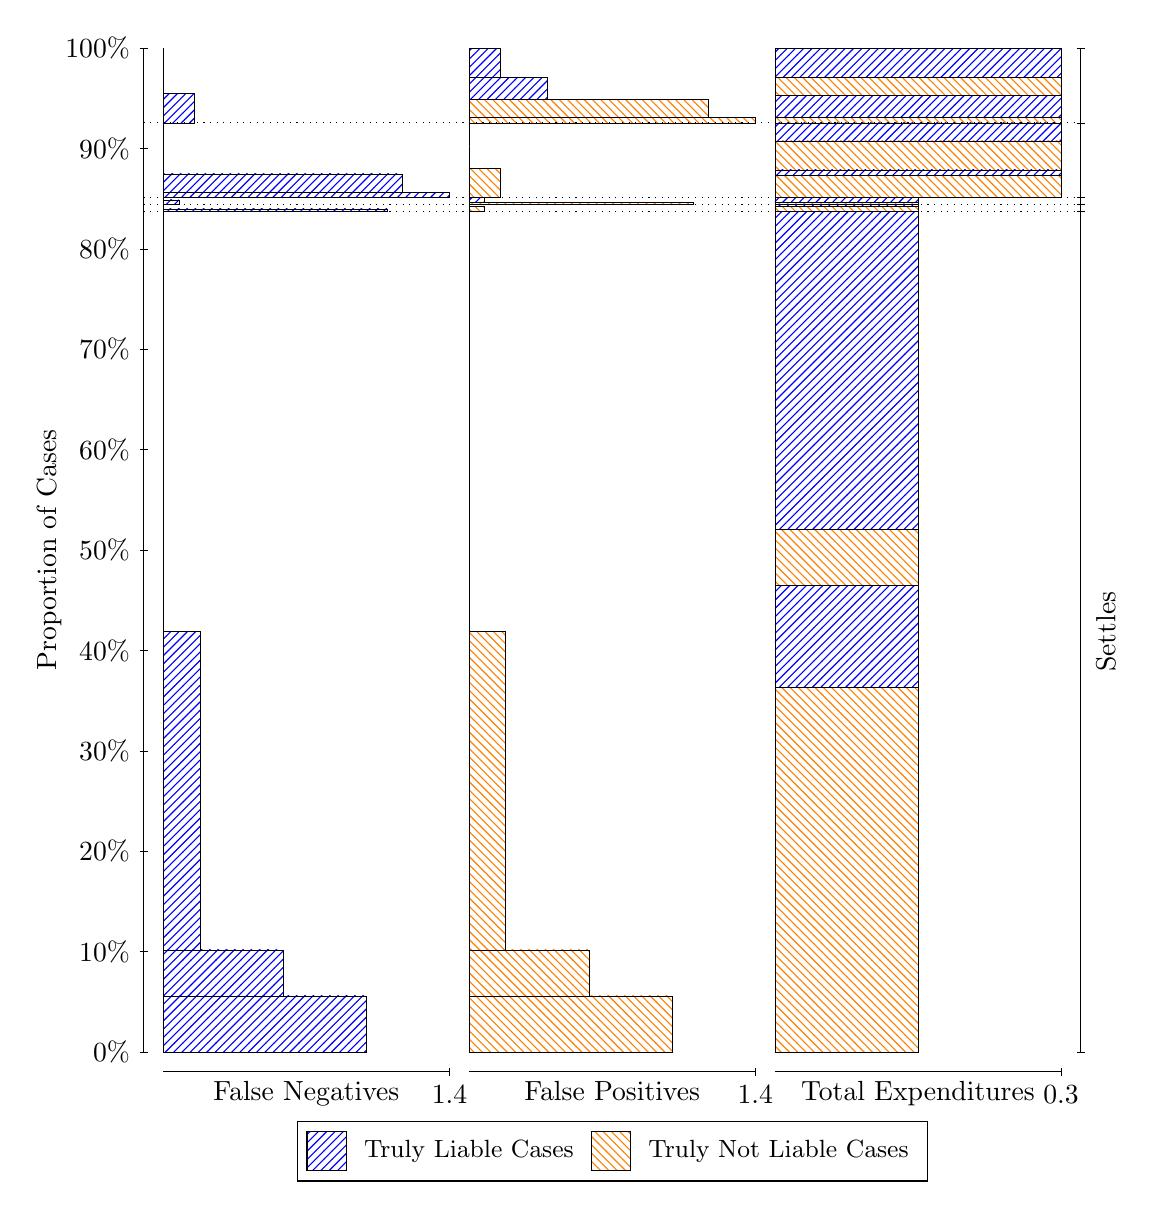
\begin{tikzpicture}
\draw[black, very thin] (1.5,1.75) -- (1.5,14.5);
\node[rotate=90, anchor=center] at (0.3, 8.125) {Proportion of Cases};
\draw[black, very thin] (1.45,1.75) -- (1.55,1.75);
\node[anchor=east] at (1.45, 1.75) {0\%};
\draw[black, very thin] (1.45,3.025) -- (1.55,3.025);
\node[anchor=east] at (1.45, 3.025) {10\%};
\draw[black, very thin] (1.45,4.3) -- (1.55,4.3);
\node[anchor=east] at (1.45, 4.3) {20\%};
\draw[black, very thin] (1.45,5.575) -- (1.55,5.575);
\node[anchor=east] at (1.45, 5.575) {30\%};
\draw[black, very thin] (1.45,6.85) -- (1.55,6.85);
\node[anchor=east] at (1.45, 6.85) {40\%};
\draw[black, very thin] (1.45,8.125) -- (1.55,8.125);
\node[anchor=east] at (1.45, 8.125) {50\%};
\draw[black, very thin] (1.45,9.4) -- (1.55,9.4);
\node[anchor=east] at (1.45, 9.4) {60\%};
\draw[black, very thin] (1.45,10.675) -- (1.55,10.675);
\node[anchor=east] at (1.45, 10.675) {70\%};
\draw[black, very thin] (1.45,11.95) -- (1.55,11.95);
\node[anchor=east] at (1.45, 11.95) {80\%};
\draw[black, very thin] (1.45,13.225) -- (1.55,13.225);
\node[anchor=east] at (1.45, 13.225) {90\%};
\draw[black, very thin] (1.45,14.5) -- (1.55,14.5);
\node[anchor=east] at (1.45, 14.5) {100\%};

\draw[black, very thin] (13.4,1.75) -- (13.4,14.5);
\draw[black, very thin] (13.35,1.75) -- (13.45,1.75);
\node[anchor=west] at (13.35, 1.75) {};
\draw[black, very thin] (13.35,12.426) -- (13.45,12.426);
\node[anchor=west] at (13.35, 12.426) {};
\draw[black, very thin] (13.35,12.514) -- (13.45,12.514);
\node[anchor=west] at (13.35, 12.514) {};
\draw[black, very thin] (13.35,12.601) -- (13.45,12.601);
\node[anchor=west] at (13.35, 12.601) {};
\draw[black, very thin] (13.35,13.55) -- (13.45,13.55);
\node[anchor=west] at (13.35, 13.55) {};
\draw[black, very thin] (13.35,14.5) -- (13.45,14.5);
\node[anchor=west] at (13.35, 14.5) {};

\draw[black, very thin, pattern color=blue, pattern=north east lines] (1.75,1.75) rectangle (4.3264,2.4611);
\draw[black, very thin, pattern color=blue, pattern=north east lines] (1.75,2.4611) rectangle (3.2694,3.0457);
\draw[black, very thin, pattern color=blue, pattern=north east lines] (1.75,3.0457) rectangle (2.2124,7.088);
\draw[black, very thin, pattern color=orange, pattern=north west lines] (1.75,7.088) rectangle (1.75,12.426);
\draw[black, very thin, pattern color=blue, pattern=north east lines] (1.75,12.426) rectangle (4.5906,12.456);
\draw[black, very thin, pattern color=orange, pattern=north west lines] (1.75,12.456) rectangle (1.75,12.514);
\draw[black, very thin, pattern color=blue, pattern=north east lines] (1.75,12.514) rectangle (1.9482,12.572);
\draw[black, very thin, pattern color=orange, pattern=north west lines] (1.75,12.572) rectangle (1.75,12.601);
\draw[black, very thin, pattern color=blue, pattern=north east lines] (1.75,12.601) rectangle (5.3833,12.67);
\draw[black, very thin, pattern color=blue, pattern=north east lines] (1.75,12.67) rectangle (4.7888,12.901);
\draw[black, very thin, pattern color=orange, pattern=north west lines] (1.75,12.901) rectangle (1.75,13.55);
\draw[black, very thin, pattern color=blue, pattern=north east lines] (1.75,13.55) rectangle (2.1464,13.919);
\draw[black, very thin, pattern color=orange, pattern=north west lines] (1.75,13.919) rectangle (1.75,14.218);
\draw[black, very thin, pattern color=blue, pattern=north east lines] (1.75,14.218) rectangle (1.75,14.5);
\draw[black, very thin, pattern color=orange, pattern=north west lines] (5.6333,1.75) rectangle (8.2097,2.461);
\draw[black, very thin, pattern color=orange, pattern=north west lines] (5.6333,2.461) rectangle (7.1527,3.0457);
\draw[black, very thin, pattern color=orange, pattern=north west lines] (5.6333,3.0457) rectangle (6.0958,7.0882);
\draw[black, very thin, pattern color=blue, pattern=north east lines] (5.6333,7.0882) rectangle (5.6333,12.426);
\draw[black, very thin, pattern color=orange, pattern=north west lines] (5.6333,12.426) rectangle (5.8315,12.484);
\draw[black, very thin, pattern color=blue, pattern=north east lines] (5.6333,12.484) rectangle (5.6333,12.514);
\draw[black, very thin, pattern color=orange, pattern=north west lines] (5.6333,12.514) rectangle (8.4739,12.543);
\draw[black, very thin, pattern color=blue, pattern=north east lines] (5.6333,12.543) rectangle (5.8315,12.601);
\draw[black, very thin, pattern color=orange, pattern=north west lines] (5.6333,12.601) rectangle (6.0297,12.969);
\draw[black, very thin, pattern color=orange, pattern=north west lines] (5.6333,12.969) rectangle (5.6333,13.251);
\draw[black, very thin, pattern color=blue, pattern=north east lines] (5.6333,13.251) rectangle (5.6333,13.55);
\draw[black, very thin, pattern color=orange, pattern=north west lines] (5.6333,13.55) rectangle (9.2667,13.62);
\draw[black, very thin, pattern color=orange, pattern=north west lines] (5.6333,13.62) rectangle (8.6721,13.85);
\draw[black, very thin, pattern color=blue, pattern=north east lines] (5.6333,13.85) rectangle (6.6242,14.132);
\draw[black, very thin, pattern color=blue, pattern=north east lines] (5.6333,14.132) rectangle (6.0297,14.5);
\draw[black, very thin, pattern color=orange, pattern=north west lines] (9.5167,1.75) rectangle (11.333,6.3772);
\draw[black, very thin, pattern color=blue, pattern=north east lines] (9.5167,6.3772) rectangle (11.333,7.6729);
\draw[black, very thin, pattern color=orange, pattern=north west lines] (9.5167,7.6729) rectangle (11.333,8.3839);
\draw[black, very thin, pattern color=blue, pattern=north east lines] (9.5167,8.3839) rectangle (11.333,12.426);
\draw[black, very thin, pattern color=orange, pattern=north west lines] (9.5167,12.426) rectangle (11.333,12.484);
\draw[black, very thin, pattern color=blue, pattern=north east lines] (9.5167,12.484) rectangle (11.333,12.514);
\draw[black, very thin, pattern color=orange, pattern=north west lines] (9.5167,12.514) rectangle (11.333,12.543);
\draw[black, very thin, pattern color=blue, pattern=north east lines] (9.5167,12.543) rectangle (11.333,12.601);
\draw[black, very thin, pattern color=orange, pattern=north west lines] (9.5167,12.601) rectangle (13.15,12.883);
\draw[black, very thin, pattern color=blue, pattern=north east lines] (9.5167,12.883) rectangle (13.15,12.952);
\draw[black, very thin, pattern color=orange, pattern=north west lines] (9.5167,12.952) rectangle (13.15,13.32);
\draw[black, very thin, pattern color=blue, pattern=north east lines] (9.5167,13.32) rectangle (13.15,13.55);
\draw[black, very thin, pattern color=orange, pattern=north west lines] (9.5167,13.55) rectangle (13.15,13.62);
\draw[black, very thin, pattern color=blue, pattern=north east lines] (9.5167,13.62) rectangle (13.15,13.902);
\draw[black, very thin, pattern color=orange, pattern=north west lines] (9.5167,13.902) rectangle (13.15,14.132);
\draw[black, very thin, pattern color=blue, pattern=north east lines] (9.5167,14.132) rectangle (13.15,14.5);
\draw[black, dotted] (1.5,12.426) -- (13.4,12.426);
\draw[black, dotted] (1.5,12.514) -- (13.4,12.514);
\draw[black, dotted] (1.5,12.601) -- (13.4,12.601);
\draw[black, dotted] (1.5,13.55) -- (13.4,13.55);
\draw[black, very thin] (1.75,1.5) -- (5.3833,1.5);
\node[anchor=north] at (3.5667, 1.5) {False Negatives};
\draw[black, very thin] (5.3833,1.45) -- (5.3833,1.55);
\node[anchor=north] at (5.3833, 1.45) {1.4};

\draw[black, very thin] (5.6333,1.5) -- (9.2667,1.5);
\node[anchor=north] at (7.45, 1.5) {False Positives};
\draw[black, very thin] (9.2667,1.45) -- (9.2667,1.55);
\node[anchor=north] at (9.2667, 1.45) {1.4};

\draw[black, very thin] (9.5167,1.5) -- (13.15,1.5);
\node[anchor=north] at (11.333, 1.5) {Total Expenditures};
\draw[black, very thin] (13.15,1.45) -- (13.15,1.55);
\node[anchor=north] at (13.15, 1.45) {0.3};

\node[black, centered, rotate=90] at (13.72, 7.0881) {Settles};





\draw (7.449999999999999,1.5) node[draw=none] (baseCoordinate) {};
\begin{scope}[align=center]
        \matrix[scale=0.5, draw=black, below=0.5cm of baseCoordinate, nodes={draw}, column sep=0.1cm]{
            \node[rectangle, draw, minimum width=0.5cm, minimum height=0.5cm, pattern=north east lines, pattern color=blue] {}; &
            \node[draw=none, font=\small] (B) {Truly Liable Cases}; &
            \node[rectangle, draw, minimum width=0.5cm, minimum height=0.5cm, pattern=north west lines, pattern color=orange] {}; &
            \node[draw=none, font=\small] (B) {Truly Not Liable Cases}; \\
            };
\end{scope}

\end{tikzpicture}
\end{document}